\NeedsTeXFormat{LaTeX2e}
\documentclass[12pt, a4paper]{book}

\usepackage[sc]{mathpazo}
\linespread{1.05}
\usepackage[Lenny]{fncychap}
\usepackage{fancyhdr}
\usepackage[utf8]{inputenc}
\usepackage{subfig}
\usepackage{epsfig}
\usepackage{epstopdf}
\usepackage{caption}
\usepackage{graphicx}
\usepackage{keyval}
\usepackage{float}
\usepackage{listings}
\usepackage{color}
\usepackage{textcomp}
\usepackage{datetime}
\usepackage[numbers, sort&compress, comma]{natbib}
\usepackage{subeqnarray}
\usepackage{longtable}
\usepackage{booktabs}
\usepackage{array}
\usepackage{amsmath}
\usepackage{amsfonts}
\usepackage{amssymb}
\usepackage [linktocpage=all]{hyperref}
\hypersetup{
  pdftitle    = {Titel},
  pdfsubject  = {Electrical Engineering},
  pdfauthor   = {Robin Weiß},
  pdfkeywords = {Bachelor Thesis} ,
  pdfcreator  = {pdflatex},
  pdfproducer = {LaTeX}
}

\usepackage[acronym, nopostdot, nonumberlist]{glossaries}
\newglossary[nlg]{notation}{not}{ntn}{Notation}

\setcounter{tocdepth}{3}
\setcounter{secnumdepth}{4}

\lhead[\fancyplain{}{\thepage}]{\fancyplain{}{\sl\nouppercase\rightmark}}
\rhead[\fancyplain{}{\sl\nouppercase\leftmark}]{\fancyplain{}{\thepage}}
\cfoot{}

\clubpenalty = 10000
\widowpenalty = 10000 
\displaywidowpenalty = 10000

\newcommand{\clearemptydoublepage}
{\newpage{\pagestyle{empty}\cleardoublepage}}

\makeglossaries
\setlength{\glsdescwidth}{0.8\linewidth}


\newglossaryentry{gls:set}{
  name=set,
  description={A collection of distinct objects}}


\newacronym{CITIC-UGR}{CITIC-UGR}{Research Centre for Information and Communications Technologies of the University of Granada}

\newacronym[description=Inertial measurement unit]{IMU}{IMU}{inertial measurement unit}

\newacronym[description=Magnetic inertial measurement unit]{MIMU}{MIMU}{magnetic inertial measurement unit}

\newacronym[description={Magnetic, angular rate, and gravity sensors}]{MARG}{MARG sensors}{Magnetic, angular rate, and gravity sensors}

\newacronym[description={Microelectromechanical systems}]{MEMS}{MEMS}{microelectromechanical systems}

\newacronym[description={Angle random walk}]{ARW}{ARW}{angle random walk}


\newglossaryentry{not:F}{
  type=notation,
  name={$\mathbf{F}$},
  description={Three-dimensional force vector},
  sort={F}}
  
\newglossaryentry{not:B_v}{
  type=notation,
  name={$\mathbf{B}$},
  description={Control matrix that relates the control input to the state $\mathbf{x}$},
  sort={Ba}}
 
\newglossaryentry{not:m}{
  type=notation,
  name={$m$},
  description={Mass},
  sort={m}}
  
\newglossaryentry{not:sigma}{
  type=notation,
  name={$\sigma$},
  description={Standard deviation},
  sort={sigma}}
  
\newglossaryentry{not:sigma_2}{
  type=notation,
  name={$\sigma^2$},
  description={Variance},
  sort={sigma}}
  
\newglossaryentry{not:mu}{
  type=notation,
  name={$\mu$},
  description={Mean value of conditional probability density},
  sort={sigma}}
  
\newglossaryentry{not:n}{
  type=notation,
  name={$n$},
  description={Discrete time},
  sort={n}}
  
\newglossaryentry{not:a}{
  type=notation,
  name={$\mathbf{a}$},
  description={Three-dimensional acceleration vector},
  sort={a}}
  
\newglossaryentry{not:impulse}{
  type=notation,
  name={$w_0, w_1, w_2, \dots$},
  description={Impulse response of a linear discrete-time filter},
  sort={wa}}
  
\newglossaryentry{not:input}{
  type=notation,
  name={$y(0), y(1), y(2), \dots$},
  description={Time series that serves as input to a linear discrete-time filter},
  sort={yaa}}
  
\newglossaryentry{not:desired_response}{
  type=notation,
  name={$d$},
  description={Desired filter response of a linear discrete-time filter},
  sort={d}}
  
\newglossaryentry{not:error_signal}{
  type=notation,
  name={$e$},
  description={Error signal of a linear discrete-time filter},
  sort={e}}
  
\newglossaryentry{not:t}{
  type=notation,
  name={$t$},
  description={Continuous time},
  sort={t}}

\newglossaryentry{not:x_v}{
  type=notation,
  name={$\mathbf{x}$},
  description={State vector of a linear dynamical system},
  sort={xb}}
  
\newglossaryentry{not:x}{
  type=notation,
  name={$x$},
  description={One-dimensional location},
  sort={x}}
  
\newglossaryentry{not:x_hat}{
  type=notation,
  name={$\hat{x}$},
  description={Estimate of $x$},
  sort={xa}}
  
\newglossaryentry{not:w_v}{
  type=notation,
  name={$\mathbf{w}$},
  description={Process noise vector},
  sort={wa}}
  
\newglossaryentry{not:v}{
  type=notation,
  name={$\mathbf{v}$},
  description={Measurement noise vector},
  sort={v}}
  
\newglossaryentry{not:u}{
  type=notation,
  name={$u$},
  description={Nominal velocity},
  sort={u}}
  
\newglossaryentry{not:w}{
  type=notation,
  name={$w$},
  description={Noise term},
  sort={w}}

\newglossaryentry{not:x_hat_v}{
  type=notation,
  name={$\hat{\mathbf{x}}$},
  description={Estimate of the state vector of a linear dynamical system},
  sort={xd}}
  
\newglossaryentry{not:x_hat_minus}{
  type=notation,
  name={$\hat{\mathbf{x}}^-_k$},
  description={A priori estimate of $\hat{\mathbf{x}}$, conditioned on all prior measurements except the one at time $t_k$},
  sort={xe}}
  
\newglossaryentry{not:y}{
  type=notation,
  name={$\mathbf{y}$},
  description={Observation vector of a dynamical system},
  sort={y}}
  
\newglossaryentry{not:z}{
  type=notation,
  name={$\mathbf{z}$},
  description={Vector of measured values},
  sort={zaa}}
  
\newglossaryentry{not:H}{
  type=notation,
  name={$\mathbf{H}$},
  description={Measurement sensitivity matrix defining the linear relationship between the state of the dynamical system and the measurements that can be made},
  sort={Ha}}
  
\newglossaryentry{not:K_v}{
  type=notation,
  name={$\mathbf{K}$},
  description={Kalman gain matrix},
  sort={Kaa}}
  
\newglossaryentry{not:K}{
  type=notation,
  name={$K$},
  description={Weighting factor},
  sort={Ka}}
  
 \newglossaryentry{not:k}{
  type=notation,
  name={$k$},
  description={Discrete time normalised to sampling interval (sample number), $k \in \mathbb{N}^0$},
  sort={k}}
  
\newglossaryentry{not:P}{
  type=notation,
  name={$\mathbf{P}$},
  description={Covariance matrix of state estimation uncertainty},
  sort={P}}
  
\newglossaryentry{not:Q}{
  type=notation,
  name={$\mathbf{Q}$},
  description={Covariance matrix of process noise in the system state dynamics},
  sort={Q}}
  
\newglossaryentry{not:R}{
  type=notation,
  name={$\mathbf{R}$},
  description={Covariance matrix of observational (measurement) uncertainty},
  sort={R}}
  
\newglossaryentry{not:phi}{
  type=notation,
  name={$\bm{\Phi}$},
  description={State transition matrix of a discrete linear dynamical system},
  sort={phiaa}}
  
\newglossaryentry{not:x_k}{
  type=notation,
  name={$\mathbf{x}_k$},
  description={The $k$th element of a sequence $\dots$, $\mathbf{x}_{k-1}$, $\mathbf{x}_k$, $\mathbf{x}_{k+1}, \dots$ of vectors},
  sort={xc}}
  
 \newglossaryentry{not:unit-delay}{
  type=notation,
  name={$z^{-1}$},
  description={Unit-delay},
  sort={za}}
  
\newglossaryentry{not:roll}{
  type=notation,
  name={$\phi$},
  description={Roll angle that determines the rotation around the $x$-axis},
  sort={phi}}
  
\newglossaryentry{not:pitch}{
  type=notation,
  name={$\theta$},
  description={Pitch angle that determines the rotation around the $y$-axis},
  sort={theta}}
  
\newglossaryentry{not:yaw}{
  type=notation,
  name={$\psi$},
  description={Yaw angle that determines the rotation around the $z$-axis},
  sort={psi}}

\newglossaryentry{not:navigation_frame}{
  type=notation,
  name={$x, y, z$},
  description={Axes of the fixed navigation frame},
  sort={xayaza}}
  
\newglossaryentry{not:body_frame}{
  type=notation,
  name={$X, Y, Z$},
  description={Axes of the moving body frame},
  sort={xayazb}}
  
\newglossaryentry{not:transformation_matrix}{
  type=notation,
  name={$\mathbf{T}$},
  description={Transformation matrix},
  sort={Ta}}
  
\newglossaryentry{not:transformation_matrix_bn}{
  type=notation,
  name={$\mathbf{C}_{bn}$},
  description={Transformation matrix transforming a position vector from the body frame to the navigation frame},
  sort={Cbn}}
  
\newglossaryentry{not:transformation_matrix_nb}{
  type=notation,
  name={$\mathbf{C}_{nb}$},
  description={Transformation matrix transforming a position vector from the navigation frame to the body frame},
  sort={Cnb}}
  
\newglossaryentry{not:omega}{
  type=notation,
  name={$\bm{\Omega}_{\mathbf{E} \rightarrow \mathbf{E}}$},
  description={Function that transforms a position vector $\mathbf{b}$ in the vector space $\mathbf{E}$ into the vector $\mathbf{b}^{'}$ in the vector space $\mathbf{E}^{'}$},
  sort={Om}}
  
\newglossaryentry{not:position_vector}{
  type=notation,
  name={$\mathbf{b}$},
  description={Position vector in a three-dimensional vector space},
  sort={b}}
  
\newglossaryentry{not:phi_vec}{
  type=notation,
  name={$\bm{\phi}$},
  description={Functional denoting the \emph{non-linear} transition matrix function of a discrete dynamical system},
  sort={phia}}
  
\newglossaryentry{not:h_vec}{
  type=notation,
  name={$\mathbf{h}$},
  description={Functional denoting the \emph{non-linear} measurement matrix function of a discrete dynamical system},
  sort={h}}
  
  
    

\begin{document}

	\frontmatter

	\begin{titlepage}
\label{ch:titlepage}
\begin{center}


\includegraphics[width=7cm]{images/universidad_de_granada.eps}
	\hfill
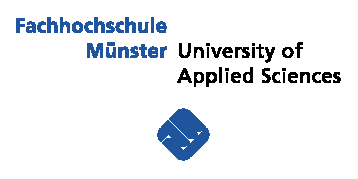
\includegraphics[width=5cm]{images/fh-muenster.eps}
	\hspace{1.0cm}
	\\ 

\vspace{3cm}

\Large\textbf{Bachelor Thesis}

\large\textsc{electrical engineering}

\vspace{1cm}

{\huge\textbf{Analysis of Anticipatory Postural Adjustments of Parkinson's Patients Using Inertial Sensors}}

\vspace{1cm}

Department of Electrical Engineering and Computer Science

\textbf{Münster University of Applied Sciences}

\end{center}

\vspace{1.5cm}

\textbf{Written by:}  \hfill \textbf{Supervised by:}

Robin Weiß \hfill Prof. Dr.-Ing. Peter Gl\"{o}sek\"{o}tter 

\hfill Ph.D. Alberto Olivares Vicente

\hfill Prof. Dr. med. Kai B\"{o}tzel

\vfill

Granada, \today

\end{titlepage}

	\clearemptydoublepage
	
	\setcounter{page}{1}	
	\phantomsection
	\addcontentsline{toc}{chapter}{Statement of Authorship}
	\thispagestyle{empty}

\section*{Statement of Authorship}
I hereby certify that this bachelor thesis has been composed by myself, and describes my own work, unless otherwise acknowledged in the text. All references and verbatim extracts have been quoted, and all sources of information have been specifically acknowledged. It has not been accepted in any previous application for a degree.

\vspace{1cm}

\noindent 
Granada, \the\day st \monthname \: \the\year

\vspace{2cm}

\noindent
Robin Weiß

	\clearemptydoublepage
	
	\phantomsection
	\addcontentsline{toc}{chapter}{Preface}
	\chapter{Preface}

This thesis was submitted in partial fulfilment of the requirements for the degree of Bachelor of Science in Electrical Engineering. It describes the implementation of a new Kalman filter based orientation algorithm to improve the estimation of orientation angles by means of inertial sensors.

I took part in the joint research project “Human Body Motion Analysis of Patients with Neurodegenerative Diseases by Means of Inertial Sensors” between the \gls{CITIC-UGR}, Spain, and the Department of Neurology of the Klinikum Großhadern, which is part of the Ludwig Maximilian University of Munich, Germany. The goal of the overall project was to obtain several gait parameters by wearable inertial sensors and validate them against conventional methods such as force plates and cameras in combination with visual markers. Physicians and medical researchers are interested in this approach of body motion analysis, as unobtrusive wearable sensors can assist the diagnosis of neurodegenerative diseases such as Parkinson's. Prior to this thesis I completed a three-months internship at the \gls{CITIC-UGR} in which I worked on the synchronisation of a force measuring plate and inertial sensors within the above-mentioned project.
	\clearemptydoublepage

	\phantomsection
	\addcontentsline{toc}{chapter}{Abstract}
	\thispagestyle{plain}
  \null\vfil
  
\begin{center}
    \setlength{\parskip}{0pt}
    {\normalsize \textsc{Münster University of Applied Sciences} \par}
    \bigskip
    {\huge{\textsc{Abstract}} \par}
    \bigskip
    {\normalsize Department of Electrical Engineering and Computer Science \par}
    \bigskip
    {\normalsize Bachelor of Science \par}
    \bigskip
    {\normalsize\bf Analysis of anticipatory postural adjustments of Parkinson's patients using inertial sensors \par} % Thesis title
    \medskip
    {\normalsize by Robin Weiß \par} % Author name
    \bigskip
  \end{center}

\noindent  
This thesis entitled ``Analysis of anticipatory postural adjustments of Parkinson's patients using inertial sensors'' was submitted in partial fulfilment of the requirements for the degree of Bachelor of Science in Electrical Engineering. 

I took part in a conjoint project between the Research Centre for Information and Communications Technologies of the University of Granada (CITIC-UGR) and the Department of Neurology of the Klinikum Großhadern in Munich, which is part of the Ludwig-Maximilians University. The objective of this thesis was to carry out an analysis of the so called anticipatory postural adjustments, which are the movements by a human subject between the moment he initiates gait and the first step.



	\clearemptydoublepage
	
	\phantomsection
	\addcontentsline{toc}{chapter}{Contents}
	\tableofcontents
	\thispagestyle{plain}
		
	\listoffigures
	\phantomsection
	\addcontentsline{toc}{chapter}{List of Figures}
	\thispagestyle{plain}
	\clearemptydoublepage

	\listoftables
	\phantomsection
	\addcontentsline{toc}{chapter}{List of Tables}
	\thispagestyle{plain}
	\clearemptydoublepage	
	
	\printglossary[type=acronym, title={Abbreviations}, style=super]
	\phantomsection
	\addcontentsline{toc}{chapter}{Abbreviations}
	\thispagestyle{plain}
	\clearemptydoublepage
    
    \printglossary[type=notation, style=super]
    \phantomsection
    \addcontentsline{toc}{chapter}{Notation}
    \thispagestyle{plain}
    \clearemptydoublepage
	
	\mainmatter
	
	\pagestyle{fancyplain}
		
	\chapter{Introduction}
\label{ch:Introduction}

\section{General}

\subsection{Parkinson's Disease}

According to Patients Medical \cite{patients_medical_definition_2014}, \begin{quote}``Parkinson's disease is a progressive, neurodegenerative disease that occurs when the neurons within the brain responsible for producing the chemical dopamine become impaired or die. Dopamine is essential for the smooth control and coordination of the movement of voluntary muscle groups. Once approximately 80\% of the brain's dopamine producing cells no longer function, the symptoms of Parkinson's disease begin to appear. [\dots] Parkinson's disease may be termed as a progressive movement disorder that is distinguished by marked slow movements, tremors, and unstable posture.''\end{quote}

Especially in advanced stages of the Parkinson's disease (PD)\nomenclature{PD}{Parkinson's disease} many patients exhibit an episodic, brief inability to step that delays gait initiation or interrupts ongoing gait. This phenomenon is called freezing of gait and is often associated with an alternating shaking of the knees, called knee trembling. However, these clinical signs of balance or gait problems are not evident in early stages of the disease \cite{mancini_anticipatory_2009}\cite{jacobs_knee_2009}.

\subsection{Anticipatory Postural Adjustments}

A major challange to the human ballance control system is the fact that we are bipeds having only one foot in contact with the ground while walking, and that two-thirds  of our body mass is located two-thirds of body height above the ground \cite{halliday_initiation_1998}. Thus, to induce stable gait anticipatory postural adjustments (APAs)\nomenclature{APAs}{Anticipatory Postural Adjustments} are necessary. The Encyclopedia of Neuroscience \cite[p.133]{woollacott_anticipatory_2009} defines APAs as "A predictive motor response that acts to counter, in a preemptive manner, the postural destabilization associated with a forthcoming movement." As seen in Figure \ref{fig:APAoverview} the centre of body mass (COM)\nomenclature{COM}{Centre of Mass} is accelerated forward and laterally over the stance foot to make sure that the body does not fall laterally toward the stepping foot during the swing phase \cite{woollacott_anticipatory_2009}.  The curve of the centre of pressure (COP)\nomenclature{COP}{Centre of Pressure} is divided in three periods. Period S1 indicates the uncoupling of the COP and COM as the COP moves posteriorly and toward the intended stepping limb. Then, in the S2 period, the COP displaces mediolaterally toward the stance foot. Finally, during the S3 period the COP moves anteriorly under the stance foot \cite{hass_gait_2005-1}.

\begin{figure}
	\centering
	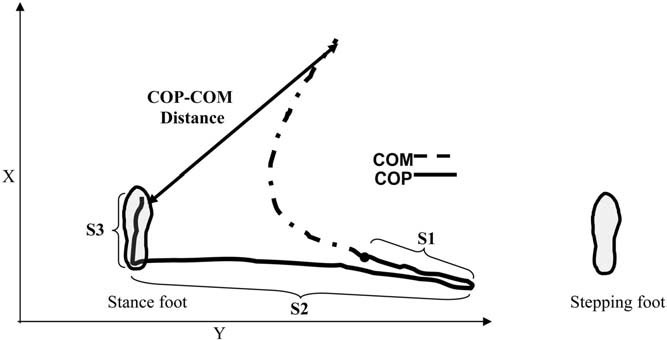
\epsfig{file=images/APA_overview, width=9cm}
	\caption{Anticipatory Postural Adjustments during forward-oriented gait initiation when stepping with the right foot \cite{hass_gait_2005-1}.}
	\label{fig:APAoverview}
\end{figure}


\section{Goals}

The goal of the project was to analyse anticipatory postural adjustments prior to step inition and subsequently build a classifier using MATLAB, which is fed with data from both a force plate and a magnetic inertial measurement unit (GaitWatch \cite{olivares_vicente_gaitwatch_2013}) to distinguish between Parkinson patients and healthy subjects. To gather the data the subject stood in front of the force plate. Then the GaitWatch and force plate record was started and the subject made a step onto the force plate. After standing a variable time of two to ten seconds the subject left the force plate, made a few steps, turned left und stopped in front of it again. This sequence was repeated ten times.


\section{Motivation}

Advanced PD can increasingly diminish quality of life, since patients are dependent on help from others to accomplish daily tasks. New drugs are currently being developed and are expected to decelerate or stop the course of the disease in early stages \cite{botzel_motivation_2014}. Thus, a quantitative PD classification enabling early diagnosis of the disease could optimise early treatment and could help to validate new treatment methods. Additionally, an objective evaluation of longterm treatment success was ensured.


\section{State of the art}

There are several methods and devices to assess Parkinson's disease and to analyse anticipatory postural adjustments. They differ in terms of practicability, accuracy, validity, portability, and cost. The state of the art at the beginning of the project is described below.

\subsection{Rating scales}

A commonly used rating scale is the Unified Parkinson’s Disease Rating Scale (UPDRS),\nomenclature{UPDRS}{Unified Parkinson’s Disease Rating Scale} which is a short test performed by a physician \cite{klerk_long-term_2009}. The patient is rated on 31 different items (see Table \ref{tab:UPDRS}) with a score of 0 (normal) to 4 (severely affected). Another method is the rough, but widely utilised and accepted Hoehn and Yahr scale (HY)\nomenclature{HY}{Hoehn and Yahr scale}. Parkinsonian motor impairment is categorised in 5 stages: Unilateral (Stage 1) to bilateral disease (Stage 2) without balance difficulties, to the presence of postural instability (Stage 3), loss of physical independence (Stage 4), up to being wheelchair- or bed-bound (Stage 5) \cite{goetz_movement_2004}. Without the need of complex technical devices these tests are relatively simple to perform. \citeauthor{klerk_long-term_2009} \cite{klerk_long-term_2009} mentioned their disadvantages, including subjectivity, short observation periods, and unfamiliarity of the environment that both rating methods bring along.

\begin{table}[h]
\begin{tabular}{lll}
\hline
Mentation, mood & Activities of daily & Motor examination \\
and behavior & living & \\
\hline
Intellectual impairment & Speech & Speech \\

Thought disorder & Salivation & Facial expression\\

Depression & Swallowing & Tremor at rest \\

Motivation/initiative & Handwriting & Action or postural tremor of hands \\

& Use of eating utensils & Rigidity \\

& Dressing & Finger taps\\

& Hygiene & Hand movements\\

& Turning in bed & Rapid alternating movements of hands\\

& Falling & Food agility\\

& Freezing when walking & Arising from chair \\

& Walking & Posture\\

& Tremor & Gait\\

& Sensory Complaints & Posture stability\\

& & Body bradikinesia and hypokinesia \\
\hline
\end{tabular}
\caption{Unified Parkinson's Disease Rating Scale items adapted from \cite{herndon_handbook_2006}.}
\label{tab:UPDRS}
\end{table}

\subsection{Instrumentation}

In addition to the aforementioned subjective rating scales, there are different devices used to quantify gait and posture and assess them objectively. All of them come with certain pros and cons. The following devices have been used:

\subsubsection{Electromyographs} Electromyography is a technique for evaluating the electrical activity of skeletal muscles. Successive action potentials generated by muscle cells are measured, by means of needle electrodes inserted into the muscles, and displayed on a cathode-ray oscilloscope. Thus medical abnormalities can be detected. The instrument used to capture the visual recording, termed electromyogram, is called electromyograph \cite{encyclopedia_britannica_electromyography_2014}. Electromyography is constrained to clinical application only, but gives indication about the contribution of specific, individual muscles to APAs.

\subsubsection{Force plates} Force plates quantify the ground reaction force (GRF)\nomenclature{GRF}{Ground Reaction Force}, which is the force exerted to the human body by the ground. The GRF is a three-dimensional vector with three orthogonal components. One component along the direction of gravity, one parallel to the ground in the sagittal plane, and one parallel to the ground in the frontal plane. Those are vertical planes that divide the body in left and right halves, and ventral and dorsal sections, respectively. A force plate usually gives an electrical voltage proportional to the force in each of the three directions. Force plates can be characterised according to the following criteria: Sensitivity in Volts per Newton, crosstalk (indication of vertical force if a horizontal force is applied and vice versa), repeatability (similar results under the same load), and time- and temperature drift \cite{griffiths_principles_2006}. Froce plates are limited to clinical application, too. They have the advantage that they don't have to be calibrated.

\subsubsection{Inertial measurement units} Devices that use a combination of inertial sensors like accelerometers and gyroscopes are referred to as inertial measurement units (IMUs)\nomenclature{IMU}{Inertial Measurement Unit}. If they also include magnetic field sensors (magnetometers), they are called magnetic inertial measurement units (MIMUs)\nomenclature{MIMU}{Magnetic Inertial Measurement Unit}. With these devices the orientation of the body can be obtained with up to nine degrees of freedom, provided that triaxial accelerometers and magnetometers are used, respectively \cite{olivares_vicente_signal_2013}.

\begin{itemize}

\item \textsc{Accelerometers} measure the acceleration of an object relative to an inertial frame. Since acceleration cannot be measured directly, the force exerted to a reference mass is obtained and the resultant acceleration is computed according to Newton's second law $ \mathbf{F} = m \cdot \mathbf a $ \cite{encyclopedia_britannica_accelerometer_2014}.

\item \textsc{Gyroscopes} measure angular velocity and are based on the Coriolis Effect. By means of integration of the angular velocity the rotation angle is obtained \cite{olivares_vicente_signal_2013}.

\item \textsc{Magnetometers} measure the strength and the direction of the magnetic field in a point in space, using the relationship between magnetic fields, movement and induced currents \cite{olivares_vicente_signal_2013}.
 
\end{itemize}
MIMUs are portable and relatively inexpensive. They can be easily attached to the body and thus allow non-clinical longterm application. Their drawbacks are complex calibration procedures and drift behaviour over time, depending on intensity and duration of the movement. Hence, in order to maintain a satisfactory degree of precision, periodical recomputation of the calibration parameters is required \cite{olivares_vicente_signal_2013}.

\subsection{Classification}

There are several research works in the literature dealing with APA analysis and PD classification, as the evaluation of posture and gait are key components of the clinical evaluation of PD \cite{palmerini_classification_2013}.

\citeauthor{klerk_long-term_2009} \cite{klerk_long-term_2009} developed a measurement system called PD Monitor, implementing an Activity Classifier that quantifies tremor and bradykinesia in the arm, thigh, and trunk, in an ambulant way and over long periods of time. They validated their measurements with video records, which were rated by physicians using the UPDRS and concluded that ``the PD monitor can be used for a detailed evaluation of the PD motor symptoms in order to optimize treatment.'' \cite{klerk_long-term_2009}.

\citeauthor{mancini_anticipatory_2009} \cite{mancini_anticipatory_2009} found that the 11 untreated early-to-middle stage Parkinson's patients that took part in their study have a significantly smaller peak COP displacement towards the stepping leg and peak trunk acceleration towards the stance leg compared to the 12 age-matched healthy control subjects. Even though step velocity and step length were not different. The results show that lateral APAs are impaired in early, untreated PD and that they are detectable with inertial sensors. As well as force plate-based, also acceleration-based extracted features can be used to detect impairments equally well. Due to the fact that the acceleration signal can be easily obtained via a sensor on a belt, no matter if in clinical or home environment, APA detection by means of accelerometers is considered as a useful way to characterise patients in early stage of PD without evident clinical symptoms. Additionally in \cite{mancini_anticipatory_2009} it is proposed to carry out further studies to determine the relationship between small APAs and the probability to develop start hesitation and freezing.

\citeauthor{palmerini_classification_2013} \cite{palmerini_classification_2013} states that PD classfication could deliver a tool to follow the progression of the disease during the entire course to examine the efficiency of treatment. They studied classification of PD subjects  using triaxial accelerometers on the lower back at L5 level and an ad hoc wrapper feature selection technique and achieved satisfactory accuracy of 93.75\%. Twenty early-mild PD subjects and 20 healthy age-matched control subjects had to perform two simple tests (quiet standing, Timed Up and Go test), in two evaluations over a 1-year follow-up, to test accuracy and robustness over time. As well as \cite{mancini_anticipatory_2009} they found that lateral dynamics i.e. range of motion are impaired in early-mild PD and suggested further investigation on validity of measures in later stages.

\section{Document structure}


	\chapter{Fundamentals}
\label{ch:Fundamentals}

\section{Inertial Measurement Units}

Devices using a combination of accelerometers and gyroscopes to measure the orientation of a solid body with up to six degrees of freedom are referred to as \glspl{IMU}. If they include magnetic field sensors (magnetometers), they are termed \glspl{MIMU}.

\glspl{MIMU} are portable and relatively inexpensive. They can be easily attached to the body and thus allow non-clinical longterm application. Their drawbacks are complex calibration procedures and drift behaviour over time, depending on intensity and duration of the movement. Hence, in order to maintain a satisfactory degree of precision, periodical recomputation of the calibration parameters is required \cite{olivares_vicente_signal_2013}.

\subsection{Accelerometers}

Accelerometers measure the acceleration of an object relative to an inertial frame. Since acceleration cannot be measured directly, the force exerted to a reference mass is obtained and the resultant acceleration is computed according to Newton's second law $ \mathbf{F} = m \cdot \mathbf a $ \cite{encyclopedia_britannica_accelerometer_2014}.

\subsection{Gyroscopes}

Gyroscopes measure angular velocity and are based on the Coriolis Effect. By integrating the angular velocity the rotation angle is obtained \cite{olivares_vicente_signal_2013}.

\subsection{Magnetometers}

Magnetometers measure the strength and the direction of the magnetic field in a point in space, using the relationship between magnetic fields, movement and induced currents \cite{olivares_vicente_signal_2013}.


\section{The Filtering Problem}

Conceived in general terms, a filter is a physical device for removing unwanted components of a mixture. In the technical field a filter is a system designed to extract information from noisy, distorted data. That is, the filter delivers an estimate of the variables of principal interest, which is why it may also be called an estimator. Filter theory is applied in diverse fields of science and technology, such as communications, radar, sonar, navigation, and biomedical engineering \cite{haykin2002adaptive}.

Consider, as an example involving filter theory, the continuous-time dynamical system depicted in Figure \ref{fig:state_estimation}. The state vector of the system, \gls{not:x(t)_v}, is usually hidden and can only be observed by indirect measurements \gls{not:y(t)_v} that are a function of \gls{not:x(t)_v} and subject to noise. Equally, the equation describing the evolution of the state \gls{not:x(t)_v} is usually subject to system errors. The dynamical system may be an aircraft in flight, in which case the elements of the state vector are constituted by its position and velocity. The measuring system may be a tracking radar producing the observation vector \gls{not:y(t)_v} over an interval $[0, T]$. The requirement is to deliver a reliable estimate \gls{not:x_hat(t)_v} of the state \gls{not:x(t)_v}, taking prior information into account.

\tikzstyle{block} = [draw, rectangle, minimum height=3em, minimum width=6em]
\tikzstyle{output} = [coordinate]
\tikzstyle{pinstyle} = [pin edge={to-, thin, black}, align=center]

\begin{figure}
\centering
\begin{tikzpicture}[auto, node distance=3cm,>=latex']
    \node [block, align=center, 
    	pin={[pinstyle]below:System \\ Errors}]
    	(dynamical) {Dynamical \\ system};
    \node [block, align=center, right of=dynamical, pin={[pinstyle]below:Measurement \\ errors}, node distance=4.5cm] (measuring) {Measuring \\ system};
    \node [block, align=center, right of=measuring, pin={[pinstyle]below:Prior \\ information}, node distance=4.5cm] (estimator) {Estimator};
    \node [output, right of=estimator] (output) {};
    
    \draw [->, align=center] (dynamical) -- node[name=x] {State \\ \gls{not:x(t)_v}} (measuring);
    \draw [->, align=center] (measuring) -- node[name=y] {Observation \\ \gls{not:y(t)_v}} (estimator);
    \draw [->, align=center] (estimator) -- node[name=y] {Estimate \\ of state \\ $\hat{\mathbf{x}}(t)$} (output);
\end{tikzpicture}
\caption{Block diagram depicting the components involved in state estimation adopted from \cite{haykin2002adaptive}.} \label{fig:state_estimation}
\end{figure}

   

\section{Digital Filters}

In contrast to analogue filters that consist of electronic circuits to attenuate unwanted frequencies in continuous-time signals and thus extracted the useful signal, a digital filter is a set of mathematical operations applied to a discrete-time signal in order to extract information about the hidden quantity of interest. A sequence of samples at equidistant time instants represent the continuous-time signal with no loss, provided the sampling theorem is satisfied, according to which the sample frequency has to be greater than twice the highest frequency component of the continuous-time signal.

Digital filters can be classified as linear and nonlinear. If the quantity at the output of the filter is a linear function of its input, that is, the filter function satisfies the superposition principle, the filter is said to be linear. Otherwise, the filter is nonlinear.

A statistical criterion according to which the performance of a filter can be measured is the mean-squared error, defined as:

$$\operatorname{MSE}=\frac{1}{n}\sum_{i=1}^n(\hat{x}_i - x_i)^2$$

\noindent
where $i$ denotes the element of the estimated state vector $\hat{\mathbf{x}}$ and the actual state vector $\mathbf{x}$ with a length of $n$, respectively. Assuming a stationary stochastic process with known statistical parameters as the mean and correlation functions of the useful signal and the unwanted additive noise, the so-called Wiener filter is said to be optimum as it minimises the mean-square value of the error signal. Since the Wiener filter requires apriori information about the statistics of the data to be processed, it may not be optimum for non-stationary processes.

\subsection{Adaptive Filters}

 

\subsection{Kalman Filters}

\section{Orientation Estimation}
	\chapter{State of the Art}
\label{ch:State_art}


	\chapter{Results and Discussion}
\label{ch:Results and Discussion}


	\chapter{Conclusion and Future Work}
\label{ch:Conclusion and Future Work}

\section{Conclusions}

%Gait analysis is a useful tool both in clinical practice and biomechanical research. In order to replace motion capture systems with low cost wearable \gls{MARG} sensors detailed technical matters still need to be improved \cite{tao_gait_2012}.
%
%Summarising the above, I can say that I have learned a lot in the four month that I spent in Granada. Amongst others I have come to know many new work methods, not only due to being exposed to people from a different culture, but also due to the fact that scientific research differs strongly from the work as a student at university. I gained a deeper understanding of orientation estimation and how Kalman filtering improves those. Therefore I had to study the principles of Kalman filters as well as the basics of MARG sensors. I was able to improve my MATLAB$\textsuperscript{\textregistered}$ skills and have realised how important it is to write understandable and well commented code, if it is for a larger project and not only for a coursework. I am now familiar with tools such as GitHub and Pivotal Tracker which make working in a team much easier and significantly more efficient.  Beside my work at the research centre, where I obtained a valuable insight into scientific research, I read a book about scientific writing that helped me to improve my oral and written English skills during my stay. Furthermore I now know the fundamentals of \LaTeX{}.
%
%All in all it was a great experience, professionally as well as personally. I truly and unreservedly recommend such a stay to \emph{every} university student.

\section{Future Work}

%Medical engineering is a very interesting blend of both my major interests, that is, working in the medical field as a paramedic and  in the technical field as an electrical engineer. There is a variety of possible future work. One related topic would be the validation of the pitch angles measured with the gyroscopes of the GaitWatch by means of cameras that record the trace of visual markers. From these markers one could compute the pitch angels and compare them to the those of the GaitWatch.



	
	\clearemptydoublepage
	\bibliographystyle{unsrtnat}
	\addcontentsline{toc}{chapter}{Bibliography}
	\bibliography{Bibliography}
	\clearemptydoublepage
	
\end{document}
